% Pour vérifier qu'on écrit du LaTeX moderne
% \RequirePackage [orthodox] {nag}

\documentclass [twoside,openright,a4paper,11pt,french] {report}

    % Règles de typographie françaises
    \usepackage[french]{babel}

    % Jeu de caractères UTF-8
    \usepackage[utf8]{inputenc}
    \usepackage[T1]{fontenc}

    % Inclure la bibliographie dans la table des matières comme une section
    \usepackage [numbib] {tocbibind}	% numbib : section numérotée

    % Fonte élégante
    \usepackage {mathpazo}
    \usepackage [scaled] {helvet}
    \usepackage {courier}

    % pour certains symboles mathématiques peu fréquents, dont \square
    \usepackage {amssymb}

    % pour \EUR
    \usepackage {marvosym}

    % \usepackage {emptypage}

    % Utilisation de tableaux
    \usepackage {tabularx}

    % Utilisation d'url
    \usepackage {hyperref}
    \urlstyle {sf}

    % Utilisation d'images
    \usepackage{graphicx}
    \setkeys {Gin} {keepaspectratio}	% par défaut : conserver les proportions

    % Définition des marges
    \usepackage [margin=25mm, foot=15mm] {geometry}

    \parskip=2mm
    \parindent=0mm

    \pagestyle {plain}

\begin{document}

%%%%%%%%%%%%%%%%%%%%%%%%%%%%%%%%%%%%%%%%%%%%%%%%%%%%%%%%%%%%%%%%%%%%%%%%%%%%%%
% Page de garde
%%%%%%%%%%%%%%%%%%%%%%%%%%%%%%%%%%%%%%%%%%%%%%%%%%%%%%%%%%%%%%%%%%%%%%%%%%%%%%

\thispagestyle{empty}

\begin{center}
    % le ".1" est juste là pour montrer qu'on peut mettre des
    % dimensions non entières...
    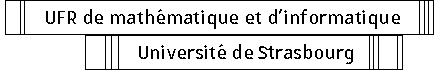
\includegraphics [width=8.1cm] {logo-ufr.pdf}       

    \vfill\vfill

    {
	\large
	\textsc {
	    Master Mathématiques et Applications\\
	    parcours Calcul Scientifique et Mathématiques de l'Innovation
	}
    }

    \bigskip\bigskip

    {\large Mémoire de stage présenté par}

    \medskip

    % Identité de l'auteur
    {\large José René \textsc {Portillo}}

    % Contact mail ou téléphone   
    {\small rene.portillo@etu.unistra.fr}

    \vfill

    % Titre du stage : mettez un titre utile
    {
	\huge
	\textsc {
	    Méthodes de détéction de fraude  \\
	    pour les assurances \\	    
	}
    }

    \vfill

    \today

    \vfill

    {\large Stage encadré par}

    \medskip

    % Identité de l'encadrant
    {\large Moisés \textsc {Rodriguez}}

    % Contact mail ou téléphone
    {\small moises.rodriguez@shift-technology.com}

    \bigskip

    {\large Au sein de}

    \medskip

    % Structure d'accueil
    {
	\large
	\textsc {SHIFT Technology}
    }

    \bigskip
    \bigskip

    % Logo de votre structure d'accueil
    
\includegraphics [height=5.5cm] {logo-entreprise.jpeg}       

    


\end{center}

% Page blanche au dos de la page de garde
%\cleardoublepage

%%%%%%%%%%%%%%%%%%%%%%%%%%%%%%%%%%%%%%%%%%%%%%%%%%%%%%%%%%%%%%%%%%%%%%%%%%%%%%
% Table des matières
%%%%%%%%%%%%%%%%%%%%%%%%%%%%%%%%%%%%%%%%%%%%%%%%%%%%%%%%%%%%%%%%%%%%%%%%%%%%%%

{
    \parskip=0pt
    \tableofcontents
}

% Page blanche entre la table des matières et le texte
\cleardoublepage

%%%%%%%%%%%%%%%%%%%%%%%%%%%%%%%%%%%%%%%%%%%%%%%%%%%%%%%%%%%%%%%%%%%%%%%%%%%%%%
% Chapitre 1
%%%%%%%%%%%%%%%%%%%%%%%%%%%%%%%%%%%%%%%%%%%%%%%%%%%%%%%%%%%%%%%%%%%%%%%%%%%%%%

\chapter {Introduction}
    \label {chap:intro}

Ce rapport a pour objectif de décrire le travail effectué durant mon stage de 
fin de master effectué entre le 3 février et le 1er août 2025. Durant ce stage,
j'ai été encadré par monsieur Moisés Rodriguez, Senior Data Scientist chez Shift Technology.

Shift Technology est une entreprise française fondée en 2014 par Jérémy Jawish, 
David Durlemman et Eric Sibony. L'objectif principal de l'entreprise est d'aider les fournisseurs
d'assurances à détecter les sinistres frauduleux. Bien que de nos jours, ils offrent d'autres 
services comme l'automatisation de processus d'assurances, la détection de documents 
et plus. 

L'entreprise compte avec plus de 500 salariés, avec 300 data scientists repartis dans le monde. En effet, basée 
dans le 12eme arrondissement de Paris, Shift Technology comporte des bureaux dans d'autres
pays comme l'Espagne, le Royaume-Uni, les États-Unis, le Mexique, le Japon et le Singapour. Les clients sont basés
dans 25 pays différents, et comportent les grands groupes de l'assurance tels que AXA, Macif ou MetLife. 

Durant ces six mois de stage, j'ai eu comme objectif de travailler dans trois tâches différentes. Premièrement, la calibration de 
scénarios déjà mit en production dans l'idée d'améliorer leur rendement et entretenir les relations avec le client pour leur présenter
le travail éffectué de façon hebdomadaire. Secondement, le déveléppement de cas de démos pour l'équipe de Go To Market, 
avec l'objectif de montrer les capacités du logiciel. Troisièmement, la mise en production d'un modèle de machine learning pour
la détection de fraude dans des sinistres avec des dégâts matériels et corporels.

%%%%%%%%%%%%%%%%%%%%%%%%%%%%%%%%%%%%%%%%%%%%%%%%%%%%%%%%%%%%%%%%%%%%%%%%%%%%%%
% Chapitre 2 : L'entreprise, le contexte, méthodes et outils
%%%%%%%%%%%%%%%%%%%%%%%%%%%%%%%%%%%%%%%%%%%%%%%%%%%%%%%%%%%%%%%%%%%%%%%%%%%%%%

\chapter {Contexte}
    \label {chap:plan}
Par la suite, c'est pertinent de donner un peu 
de contexte du monde des assurances, du produit logiciel développé par Shift Technology et comment
celui-ci fonctionne, et finalement donner les outils techniques ou logiciels qui ont été
nécessaires au cours du stage. 
\section{L'Assurance}

L'assurance est un service donné aux particuliers ou aux entreprises, dans le 
cas qu'une éventualité non désirée arrive, appelée \textbf{sinistre}. Le 
contrat d'assurance est délimité par une \textbf{police d'assurance}. Cette dernière
explicite les dédommagements à couvrir dans le cas d'un sinistre, les cas dans lequel ce 
sinistre est couvert et les primes mensuelles ou annuelles à verser au fournisseur. 

L'assurance est un produit très varié~; on peut, de manière générale, assurer deux choses~:
les biens et les personnes. Pour les biens, on utilise la dénomination \textbf{Property \& Casualty} (PnC) 
pour désigner les produits qui couvrent les voitures, les biens immobiliers ou encore les bureaux. 
En cas de sinistre entraînant la perte totale ou partielle d'un bien, cela peut donner lieu à une 
compensation monétaire ou au remplacement de la propriété.\\

La partie \emph{Casualty} fait référence à la responsabilité civile que peut encourir un assuré lorsqu'il
est reconnu fautif dans un accident. Par exemple, en cas d'accident de voiture impliquant des blessés ou 
des dommages causés aux biens d'autrui, l'assurance peut prendre en charge les frais correspondants.
 
Pour les produits liées aux les personnes ou la santé on utilise la dénomination
\textbf{Health\&Life} (H\&L). Ces produits peuvent couvrir les frais médicaux, les traitements, 
les consultations, une indemnisation dans le cas où la maladie entraine l'arrêt permanent de travail,
ou une indemnisation dans l'éventualité d'un décès. Les maladies, causes et dédommagements possibles sont 
strictement encadrés par le contrat d'assurance. 

Une fois le sinistre arrivé, pour recevoir la compensation l'assuré doit effectuer une déclaration
de sinistre ou \textbf{insurance claim}. La déclaration arrive chez un expert en sinistres qui va faire 
une investigation et une évaluation pour déterminer si l'assurance devrait payer pour les 
dédommagements, et de combien. 

\section{La fraude à l'assurance}

La fraude à l'assurance est l'acte de mentir ou décevoir le fournisseur d'assurance
soit dans la déclaration du sinistre, soit dans la conception du contrat d'assurance. 
Ainsi, celle-ci arrive, quand l'assuré reçoit des compensations que normalement 
ne seraient pas octroyées. 

Deux types de fraudes peuvent être décris:

\begin{itemize}
    \item \textbf{Fraude dure} C'est le fait d'inventer un sinistre ou des 
     dégâts non-existants. De même c'est d'effectuer un sinistre
     de façon réfléchi et prémeditée. Par exemple, en créant une collision de voiture,
    en mettant en scène un vole, ou en produisant un incendie. 

    \item \textbf{Fraude simple} C'est le fait d'exagérer les dégâts ou les 
    blessures d'un sinistre qui a vraiment eu lieu, mais ne se sont pas produits comme l'assuré 
    le dépeint. Il se produit aussi quand l'assuré profite du sinistre pour faire passer
    comme dégâts des problèmes qui précedaient le sinistre ou parfois même le contrat d'assurance. 

\end{itemize}

En France, la fraude aux assurances coûte 2 milliards d'euros aux entreprises. Au-delà du privé, 
la fraude coûte aussi de l'argent au contribuable via la fraude à la sécurité sociale, qui elle estestiméé 
à 110 milliards d'euros. 

Ainsi, Shift Technology analyse les déclaration de sinistres des entreprises clientes 
et via des modèles d'intelligence artificielle, elle permet d'émettre une alerte pour 
l'expert en sinistres pour porter une attention particulière sur un sinistre qui pourrait être de la fraude.



\section {Présentation de l'organisme d'accueil}

J'ai rejoint Shift Technology en tant que data scientist, un rôle central dans 
la conception des produits de l'entreprise. Chez Shift, les data scientists — 
appelés « DS » — sont organisés par régions géographiques. La direction globale
des DS est assurée par M. Arnaud Grapinet. La région Europe-Amériques est quant
à elle supervisée par M. Maxime Paul, tandis que les DS dédiés à l'Amérique 
latine et à l'Espagne travaillent sous la direction de Mme Sabrina Maldonado.

Les data scientists interagissent directement avec les clients ainsi qu'avec les 
experts en détection de fraude. À ce titre, la maîtrise native de la langue de la 
région concernée — l'espagnol, dans ce cas — est essentielle pour assurer une 
communication fluide et efficace.

\section {Force - La solution de détection de fraude}

\subsection{Le logiciel}
Le produit principal chez Shift est Force, un logiciel web qui aide les experts 
en sinistres à détecter la fraude. Le client s'identifie et des alertes sont 
envoyés pour les sinistres, clients ou intermédiaires suspicieux. 

La solution Force s'adapte aux besoins précis du client, aux données et son format, 
les types de fraudes et les éléments que le client veut privilégier pour alerter.
Malgré que plusieurs éléments de codes et la méthodologie soient les mêmes,
la solution n'est pas en "prêt à porter", elle est taillé et fait en fonction
du client. 

Lever une solution pour un client requiert différentes étapes, qu'on élucidera au cours de ce chapitre. 

\subsection{Mapping}

Le \textit{mapping} constitue la première étape du projet. Il s'agit de transformer les données brutes fournies par le client en un modèle prédéfini par Shift.  
Comprendre en amont les données du client est essentiel~: leur provenance, leur organisation, leur nature (par exemple, si elles sont fournies directement par les assurés), etc.

Les données sont généralement transférées via SFTP, d'un serveur du client vers un serveur de Shift. Elles alimentent ensuite une base de données appelée \textbf{Raw Model}.  
L'objectif est alors de transformer ce \textit{Raw Model} en un \textbf{Data Model} structuré et exploitable.

\begin{figure}[htbp]
    \centering
    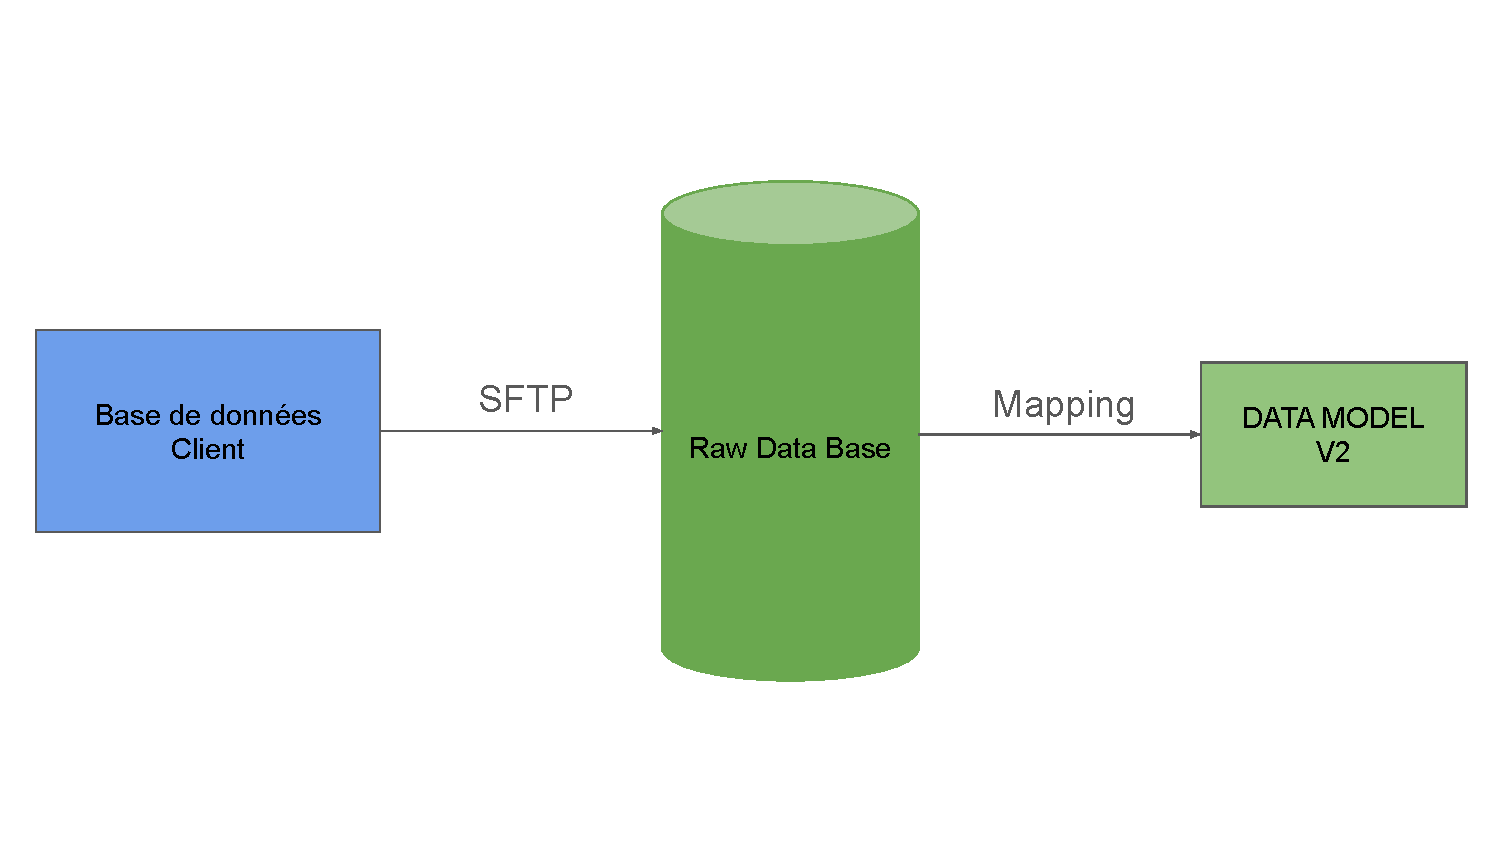
\includegraphics[width=0.80\textwidth]{Mapping.pdf}
    \caption{Transfert des donées et mapping.}
    \label{fig:entonnoir}
\end{figure}

Le \textbf{Data Model} repose sur une organisation spécifique, structurée en trois types de tables~:

\begin{itemize}
    \item \textbf{HUBS}~: les hubs contiennent des informations clés sur des entités précises, telles que la déclaration d'un sinistre, une police d'assurance, un véhicule, ou un assuré.  
    Dans le data model, un hub correspond à une table SQL qui regroupe le strict minimum d'informations nécessaires sur une entité.  
    Par exemple, dans la table \texttt{Policy}, on trouvera uniquement des éléments comme \texttt{PolicyNumber} et \texttt{PolicyOwner}.

    \item \textbf{SPECIALIZATIONS}~: ces tables contiennent les détails complémentaires d'un hub.  
    Par exemple, dans une table de spécialisation liée à un assuré, on retrouvera le nom complet, la date de naissance, l'adresse, etc.

    \item \textbf{LINKS}~: un link représente la relation entre deux hubs.  
    La table de lien contient les clés primaires des deux hubs qu'elle relie, ce qui permet d'effectuer des \texttt{JOINs} entre eux.
\end{itemize}

\subsection{Denoising et Reconstruction}

Le denoising nous aide à trouver détécter et corriger des anomalies dans les données. En effet, 
un des enjeux est de savoir si deux individus avec des données légérement différentes
sont les mêmes ou pas. Les discrépances peuvent venir de toutes les formes possibles,
une faute d'orthographe,oubli d'une lettre muette, répétition d'un mots, etc. Ainsi, 
imposer que deux individus sont les mêmes que par l'égalité stricte de tous les champs
est une règle beaucoup trop stricte et serait un obstacle à la reconstruction d'identités.
La solution à ce problème consiste à nettoyer les données en effectuant des modifications, comme 
par exemple: enlever les espaces, passer à un texte phonétique, supprimmer les 
caractères spéciaux.

Une fois les données netoyées, les "entités" (une personne, un véhicule, une organisation) seront reconstruites.
Ce qui nous permettra d'avoir un historique des "entités" liées au sinistres, et établir des liasons entre eux.

\subsection{Scénarios et détéction de fraude}

Par la suite les données seront traités par des algorithmes spécifiques qu'on appelle 
des scénarios. Un scénario de fraude correspond à un comportement frauduleux précis et défini
avec le client en amont et avec son équipe de gestionnaires de fraude.

Les scénarios analysent les données ou une partie des données et lancent des alertes 
sous certaines contraintes.  On retrouve globalement deux types de scénarios\\

\textbf{- Rule Based Scenario: } Il s'agit de scénarios qui déclenchent une alerte si, et seulement si, certaines conditions sont remplies.  
Les conditions à remplir sont nommées des \textbf{variables primaires} et sont souvent des conditions booléennes. 
Par la suite, on a des \textbf{variables secondaires ou explicatives} qui aidents les gestionnaires de fraude 
a mieux comprendre la suspicion.   
On retrouve des scénarios standards valables pour tous les clients et toutes les régions géographiques, mais qui sont paramétrés spécifiquement pour chaque client.

L'exemple le plus parlant est celui du scénario de souscription récente~: une alerte est déclenchée lorsqu'un assuré déclare un sinistre quelques jours seulement 
après la souscription du contrat d'assurance.  
Ce type de situation peut faire naître un soupçon quant à la possibilité que le sinistre soit survenu avant l'entrée en vigueur de la police.  
Cependant, les paramètres — comme le seuil de jours à partir duquel le scénario est déclenché — varient d'un client à l'autre. Tous ces détails 
sont éclaircis en amont de la mise en production. 

Un scénario spécifique, lié à la géographie et au client, peut être la détection de véhicules au Mexique provenant des États-Unis,  
acquis via des sites d'enchères, et sur lesquels on observe sur les photos, des dommages antérieurs.  
Ce genre de scénarios peut être développé en aval de la mise en production, en fonction des spécificités du client. 

Les scénarios basés sur règles sont extrêmement importants, puisqu'en fonction des règles on a un soupçon très clair et précis 
qui peut aider fortement les investigateurs de sinistres, et donner un chemin pour l'investigation. \\


\textbf{- Machine Learning Scenarios}
Il s'agit de scénarios entièrement basés sur des modèles de machine learning, en particulier sur des algorithmes d'apprentissage supervisé.  
Ces modèles sont entraînés à partir des données historiques du client, incluant notamment les sinistres identifiés comme frauduleux.  
Une fois le modèle entraîné, un score de probabilité de fraude est attribué à chaque nouveau sinistre.  
Un seuil de déclenchement est ensuite défini~: si le score dépasse ce seuil, une alerte est générée.

Le développement de ce type de scénario présente plusieurs défis.  
Tout d'abord, le nombre de cas de fraude confirmés est généralement très faible par rapport à l'ensemble des sinistres,  
ce qui crée un fort déséquilibre de classes. Ce déséquilibre rend l'entraînement des modèles plus complexe et nécessite souvent  
le recours à des techniques spécifiques telles que le sur-échantillonnage, le sous-échantillonnage ou l'utilisation de métriques adaptées  
(AUC, F1-score, etc.) pour évaluer les performances.

Ensuite, contrairement aux scénarios basés sur des règles, ceux issus du machine learning ne reposent pas sur des signaux clairs et compréhensibles pour l'utilisateur final.  
Le client se retrouve souvent sans hypothèse initiale ou élément tangible pour orienter son enquête.  
Malgré tout, ces scénarios permettent de détecter des fraudes qui auraient passé inaperçus pour l'œil humain. 




\subsection{Mise en production}

Une fois tous ces éléments mis en place, on peut commencer à recevoir les sinistres et les données du client de façon 
journalière. Le traitement et analyse sont effectuées dans les heures qui suivent, et les enquêteurs de sinistres peuvent se connecter 
à une interface graphique où on retrouve toutes les alertes avec un score spécifique pour faire le tri de façon plus efficace. 

\begin{figure}[htbp]
    \centering
    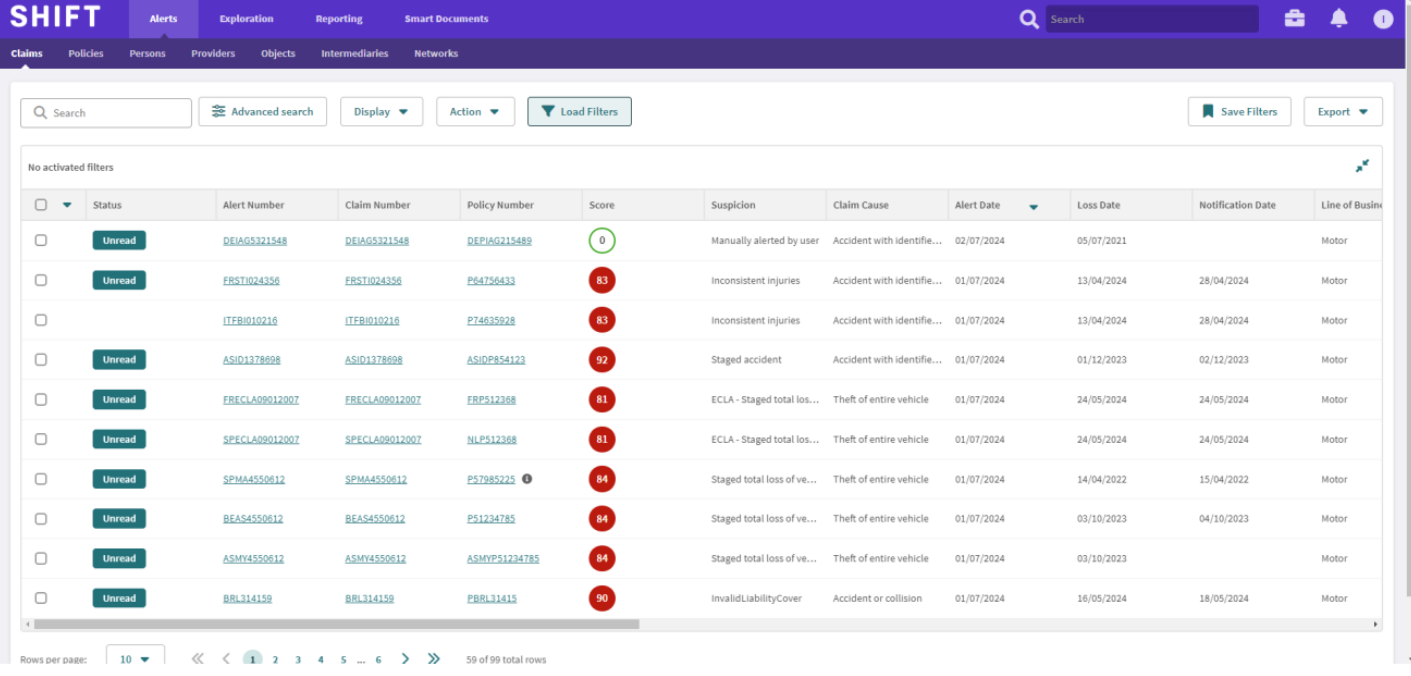
\includegraphics[width=0.80\textwidth]{interfacegraphique.png}
    \caption{Interface  Graphique de Force}
    \label{fig:entonnoir}
\end{figure}





\section{Méthodes, outils et logiciels}
\subsection*{Outils et technologies utilisés}

Au cours de ce stage, j'ai eu l'opportunité de travailler sur des projets variés, nécessitant la mobilisation de plusieurs technologies, langages de programmation et outils professionnels.

\begin{itemize}
    \item \textbf{Langages de programmation} : Le développement back-end du logiciel \textit{FORCE} est majoritairement en \textbf{C\#}, donc ceci a constitué 
    le langage principal de ce stage. Par ailleurs, l'ensemble des travaux relatifs à l'intelligence artificielle et à l'apprentissage automatique a été mené en \textbf{Python}, en s'appuyant 
    sur des bibliothèques standards telles que \textit{NumPy}, \textit{pandas}, \textit{matplotlib} et \textit{LightGBM}.
    
    \item \textbf{Stockage et traitement des données} : Le stockage des données ainsi qu'un prétraitement partiel ont été effectués à l'aide de \textbf{SQL Server}.
    
    \item \textbf{Environnement de développement (IDE)} : L'IDE principal utilisé était \textbf{JetBrains Rider}, offrant une intégration fluide avec les différents composants de l'écosystème .NET, ainsi que des outils de débogage avancés.
    
    \item \textbf{Contrôle de version} : Le suivi des versions et la gestion collaborative du code ont été assurés via \textbf{Git}, avec l'assistance de l'interface graphique \textbf{Git Extensions}.
    
    \item \textbf{Intégration et déploiement continus} : Les outils \textbf{TeamCity} et \textbf{Octopus Deploy} ont été employés pour automatiser les processus d'intégration continue et de déploiement.
\end{itemize}


\section {Les missions}

Les missions au cours du stage furent

\begin{itemize}
    \item \textbf{Création, amélioration et calibration de scénarios classiques} : Chez Shift, la plupart
     des data scientists sont assignés à un ou plusieurs clients. Leur mission principale consiste à assurer
      le suivi de la solution logicielle, développer des scénarios adaptés et les présenter aux clients.
       Dans ce cadre, j’ai apporté un appui à mon encadrant de stage sur des projets impliquant trois clients d’Amérique latine.
       J'ai donc participé à l'amélioration et correction de nombreux scénarios, et au suivi du client.
    
    \item \textbf{Machine Learning} : J’ai entraîné plusieurs modèles pour deux clients en Espagne. Ce travail comprenait 
    la génération de jeux de données, le prétraitement des variables, 
    la détection de fuites (\textit{leakage}) dans les données, l’entraînement des modèles ainsi que leur mise en production.
    
    \item \textbf{Développement de cas démos} : J’ai collaboré avec l’équipe \textit{PreSales} dans le développement
     de quinze cas démos, destinés à illustrer les capacités techniques de la solution auprès de clients potentiels.
\end{itemize}



\chapter{Les missions}
\label {chap:contexte}
\section{Amélioration et création de scénarios}

Les scénarios sont au cœur de la solution de Shift. Une fois les données correctement 
mappées, les scénarios analysent les sinistres et, si certaines conditions sont 
remplies, une alerte est envoyée au client. On appelle \textbf{alert rate} le 
pourcentage d'alertes envoyées par sinistres analysés. À partir du nombre d'alertes 
envoyées, on obtient le \textbf{taux de transformation}, qui correspond au 
pourcentage d'alertes s'avérant être des fraudes.

Ainsi, l'objectif est d'envoyer le moins d'alertes possible (réduire les faux 
positifs), tout en garantissant que les alertes envoyées soient effectivement 
frauduleuses (améliorer la précision). Pour réduire le nombre d'alertes, il est 
souvent nécessaire d'effectuer une calibration des scénarios, c'est-à-dire de modifier 
les conditions d'alertement.

Plusieurs modifications ont été apportées en collaboration avec le client au cours du 
stage. Voici une liste non exhaustive des ajustements effectués :

\begin{itemize}
    \item Augmentation de l'alertement pour les véhicules haut de gamme dans plusieurs 
          scénarios.
    \item Réduction, voire suppression, de l'alertement pour les véhicules appartenant 
          à une même entreprise ou bénéficiant d'un contrat d'assurance spécifique.
    \item Diminution de l'alertement pour les véhicules ayant passé un contrôle 
          technique récent.
    \item Élargissement des conditions du scénario lié à une souscription récente.
\end{itemize}

Une fois les modifications implémentées dans le code, une analyse d'impact est 
nécessaire afin d'évaluer l'effet de ces changements sur la performance des 
scénarios. Par exemple : si l'on diminue l'alertement, perd-on des cas de fraude ? 
Si l'on élargit les conditions pour générer plus d'alertes, observe-t-on une hausse 
des faux positifs ? Et surtout, dans quelle mesure ces ajustements sont-ils 
pertinents pour le client ?

L'analyse est effectuée à partir des sinistres enregistrés au cours des six derniers 
mois. Elle permet de présenter au client les éléments suivants :

\begin{itemize}
    \item L'évolution du taux d'alertement.
    \item L'évolution du taux de transformation.
    \item Le nombre estimé de fraudes supplémentaires détectées ou, au contraire, 
          perdues.
\end{itemize}

Dans le cas du scénario lié à une souscription récente, les conditions d'alertement 
ont été élargies. Sur 144\,000 sinistres analysés en trois mois, le nombre d'alertes 
est passé de 112 à 146, tandis que les fraudes détectées sont passées de 3 à 6.

Au cours du stage, nous avons réalisé en moyenne une calibration par semaine.

Cependant, modifier les scénarios existants ne suffit pas. En début de trimestre, 
des actions sont définies pour effectuer des modifications majeures ou pour créer de 
nouveaux scénarios à partir de zéro. Voici deux exemples de scénarios que j'ai 
développés au cours de ce stage.

\section {Votre contribution}

C'est la principale partie de votre mémoire : vous devez présenter votre
contribution (réalisation logicielle, système informatique, état de
l'art, méthode, algorithme, évaluation, etc.) de façon synthétique,
sans sombrer dans les détails techniques mais en n'éludant pas les
points concrets qui permettent au rapporteur d'avoir la vision la plus
exacte possible de ce que vous avez mis en œuvre. Ne passez pas
les difficultés auxquelles vous avez été confronté sous silence.

Soyez précis et factuel : technologies, algorithmes ou méthodes
employés, éléments quantitatifs permettant d'apprécier l'envergure
du projet, comparatifs réalisés, etc. Si vous avez travaillé en
coopération avec d'autres personnes (votre maître de stage, d'autres
personnes ou stagiaires), indiquez avec précision votre rôle et vos
réalisations.

La méthodologie avec laquelle vous procédez est l'un des principaux
critères d'évaluation de votre travail : les problèmes doivent
être analysés, les choix effectués (ou auxquels vous avez pris part)
doivent être explicités et justifiés.

Il arrive souvent que, comme stagiaire, les choix vous soient imposés :
vous vous insérez dans un contexte qui existait avant votre arrivée,
certains choix sont faits en amont ou implicitement. Vous devez
les expliciter, et montrer que vous en maîtrisez les tenants et les
aboutissants : en d'autres termes, vous devez justifier certains choix,
même si ce ne sont pas les vôtres, pour montrer votre compréhension
des enjeux.

\section {Votre bilan}

Le stage complète votre formation : vous devez prendre du recul pour
mettre en rapport votre stage avec les compétences acquises pendant votre
formation, et présenter les compétences complémentaires (techniques,
personnelles, comportementales, etc.) que vous avez acquises durant
le stage.

Le bilan doit montrer votre recul par rapport au stage : vous avez le
droit (voire le devoir) de jeter un regard personnel et critique sur
votre comportement, sur votre démarche, sur votre réalisation ou même
sur le contexte, les choix effectués ou l'organisme d'accueil.


%%%%%%%%%%%%%%%%%%%%%%%%%%%%%%%%%%%%%%%%%%%%%%%%%%%%%%%%%%%%%%%%%%%%%%%%%%%%%%
% Chapitre 3
%%%%%%%%%%%%%%%%%%%%%%%%%%%%%%%%%%%%%%%%%%%%%%%%%%%%%%%%%%%%%%%%%%%%%%%%%%%%%%

\chapter {La forme}
    \label {chap:contexte}

Un bon mémoire allie un fond de qualité et une forme parfaite. Quelques
règles de bon sens s'appliquent.

\section {Typographie}

La rédaction de textes obéit à des règles précises en
Français : cela s'appelle la «~typographie~» \cite{andre1990} et il
est intéressant de s'en imprégner pour donner à votre document un
aspect de qualité et éviter des erreurs grossières.

\section {L'orthographe et la grammaire}

L'orthographe et la grammaire sont des prérequis indispensables pour
la rédaction du mémoire. Si vous n'êtes pas sûr de vous, faites-vous
relire par un tiers. C'est dommage de perdre des points sur ce critère.

\section {Le style}

Même si votre mémoire de stage n'a pas comme objectif de décrocher
le prix Goncourt, vous devez faire attention au style :

\begin {itemize}
    \item faites des phrases construites, avec des verbes. Exemple vécu,
	à éviter : «~Il y a des problèmes. Par exemple le
	format~» (il n'y pas de verbe)~;

    \item ne parlez pas au lecteur. Exemple vécu, à éviter : «~je vais
	vous présenter~»~;

    \item employez une forme active : plutôt qu'écrire «~xyz a été
	réalisé~», utilisez «~j'ai réalisé xyz~»~;

    \item soyez précis : écrivez «~j'ai réalisé xyz~» plutôt que «~on a
	réalisé xyz~». N'oubliez pas que le rapporteur doit évaluer
	\textbf{votre} travail (et pas celui de votre maître de stage ou
	de vos collègues)~;

    \item évitez les mots inutiles («~la société xyz existe
	\emph{maintenant} depuis 1789~») ou, pire encore, les phrases
	inutiles («~au cours de ce stage, j'ai pu travailler avec
	plusieurs personnes dans quelques environnements divers et
	variés~»)~;

    \item dans la même lignée, n'abusez pas du pouvoir~: «~j'ai pu
	faire...~» est une tournure inutilement compliquée qui est
	remplaçable par «~j'ai fait...~». C'est la même chose pour le
	verbe «~permettre~», le plus souvent inutile~: «~le logiciel
	permet de faire...~» est remplaçable par la forme plus directe
	«~le logiciel fait...~».

    \item évitez le futur : tout ce qui est fait au moment de l'écriture
	du mémoire doit être rédigé au passé ou au
	présent. Réservez le futur pour ce qui n'est pas encore
	réalisé ou pour les perspectives.

\end {itemize}


\section {Numérotez}

Numérotez tout ce qui peut l'être : pages, chapitres, sections, figures,
tables, bibliographie. Laissez à votre logiciel le soin de numéroter
automatiquement, il le fera mieux que vous «~manuellement~». Utilisez
des références si vous devez mettre en relation plusieurs éléments
de votre discours (exemple fictif : voir la figure~\ref {fig:entonnoir}
page~\pageref {fig:entonnoir}, ou encore le chapitre~\ref {chap:plan}
et plus spécifiquement la section~\ref {sec:mission}, page~\pageref
{sec:mission}).


\section {Les illustrations}

Un petit dessin valant mieux qu'un grand discours, les schémas de
principe sont très appréciés par le rapporteur qui ne connaît
pas votre environnement. Quelques règles cependant sont à respecter :

\begin {itemize}
    \item numérotez et légendez vos figures (voir figure~\ref
	{fig:entonnoir}, page~\pageref {fig:entonnoir}, par exemple) ;
    \item référencez vos figures : une figure non référencée dans le
	texte ne sert à rien ;
    \item expliquez vos figures dans le texte : si une figure ne nécessite
	pas d'explications, cela signifie qu'elle est sans doute trop
	simple et n'a donc pas besoin de figurer dans votre mémoire ;
    \item la bonne taille pour les figures est celle où les caractères
	sont à peu près de la même taille que le reste du texte~;
    \item citez la provenance de vos figures, si elles ne sont pas de
	vous : il est parfaitement admis d'utiliser des figures
	réalisées par d'autres, si vous citez la provenance ;
    \item les logos de logiciels ou de produits sont à bannir : ils
	n'apportent rien à la compréhension de votre mémoire et ne font
	que prendre de la place inutile que vous pourriez utiliser pour
	mieux présenter votre contribution ;
    \item privilégiez (sauf peut-être pour les photos) un format
	«~vectoriel~» à un format «~bitmap~» : le bitmap prend
	de la place, peut être lent à s'afficher ou à s'imprimer,
	et ne permet pas de zoomer facilement ;
    \item vérifiez que vos figures sont lisibles lorsque vous imprimez
	votre mémoire, y compris lorsque vous imprimez sur une
	imprimante noir et blanc.
\end {itemize}

Les copies d'écran n'apportent généralement pas grand-chose : elles
contiennent trop d'informations inutiles et sont peu lisibles. De plus,
le message véhiculé est souvent très succinct, voire trop léger. Un
fichier de configuration, une commande ou son résultat doivent être
présentés, si c'est vraiment nécessaire, comme du texte et non comme
une copie d'écran.

\section {Le niveau de détail}

Trouver le bon niveau de détail est souvent facilité par les contraintes
qui vous sont imposées quant au nombre de pages.

Cependant, même si vous avez la place, évitez les recopies de code ou de
commandes. Si vous voulez vraiment en faire, commentez-les dans le texte
et évitez de faire des erreurs dans les recopies ! Ne les modifiez pas
dans le texte (sauf pour supprimer une sortie trop longue par exemple,
dans ce cas remplacez la partie supprimée par «~[...]~»). Évitez
les codes trop longs~: utilisez des annexes si nécessaire.


\section {La bibliographie}

La bibliographie constitue une partie importante de votre mémoire.
Elle constitue un critère de qualité du travail (avez-vous trouvé les
bonnes sources ? les documents sur lesquels vous vous appuyez sont-ils
sérieux ?). Vous devez indiquer les documents :

\begin {itemize}
    \item de référence que vous avez consultés dans votre recherche,
	pour vous familiariser avec votre sujet ou pour apprendre
	des techniques particulières ;
    \item que vous avez consultés pour effectuer vos choix ou mettre
	en œuvre un dispositif logiciel ou autre ;
    \item qui permettent au lecteur d'en savoir plus sur tel ou tel
	point de votre mémoire que vous ne pouvez davantage développer.
\end {itemize}

La bibliographie~\cite {savoirs2010} vient en annexe, elle doit donner
tous les renseignements nécessaires pour permettre au lecteur de
retrouver les documents concernés : auteur, titre du document ou de
l'ouvrage, éditeur, année de publication, URL si nécessaire, date de
consultation pour un site Web, etc.

Chaque document dans la bibliographie comporte une référence (un
numéro, une abréviation ou autre), que vous devez citer dans le texte :
un document non cité ne devrait pas apparaître dans la bibliographie.

%%%%%%%%%%%%%%%%%%%%%%%%%%%%%%%%%%%%%%%%%%%%%%%%%%%%%%%%%%%%%%%%%%%%%%%%%%%%%%
% Conclusion
%%%%%%%%%%%%%%%%%%%%%%%%%%%%%%%%%%%%%%%%%%%%%%%%%%%%%%%%%%%%%%%%%%%%%%%%%%%%%%

\chapter {Conclusion}
    \label {chap:conc}

Il est maintenant temps de rédiger votre mémoire, en vous aidant des
listes de points à vérifier dans les annexes \ref{checklist-mem} et
\ref{checklist-sout}. Puissent ces quelques
conseils vous guider afin de vous aider à présenter le mieux possible
tout le travail que vous avez effectué durant votre stage !


%%%%%%%%%%%%%%%%%%%%%%%%%%%%%%%%%%%%%%%%%%%%%%%%%%%%%%%%%%%%%%%%%%%%%%%%%%%%%%
% Annexe : soutenance
%%%%%%%%%%%%%%%%%%%%%%%%%%%%%%%%%%%%%%%%%%%%%%%%%%%%%%%%%%%%%%%%%%%%%%%%%%%%%%

\appendix
\chapter {La soutenance}

Même si ce document concerne en priorité votre mémoire de stage,
il n'est pas inutile de rappeler quelques conseils de bon sens
pour que votre soutenance se déroule le mieux possible.

\begin {enumerate}
    \item Ne reproduisez pas le mémoire dans votre présentation : vous
	n'avez ni la place, ni le temps. Détachez-vous du mémoire et
	repartez de zéro pour construire un nouveau discours tenant
	compte de la contrainte de temps.

    \item Travaillez sur les idées et les messages que vous voulez
	faire passer. Comptez une idée par diapo. Explicitez les idées,
	ne vous contentez pas de les suggérer.

    \item Ne surchargez pas le texte de votre présentation : ne faites
	pas de phrases, insistez plutôt sur quelques mots pour exposer
	vos idées.

    \item Si vous pouvez prendre des libertés avec la grammaire et
	ne pas mettre de phrases, vous n'êtes pas dispensé de respecter
	l'orthographe.

    \item Adoptez un fond sobre pour ne pas perturber votre message.
	Numérotez vos diapos.

    \item Faites des illustrations (schémas, figures, courbes) qui
	puissent être lues à plusieurs mètres de distance. N'hésitez
	pas à prendre des libertés avec votre style de présentation
	pour faire une figure en pleine page.

    \item Attention aux contrastes : votre présentation projetée dans
	une salle éclairée aura un contraste beaucoup moins bon que
	l'écran de votre portable. Évitez donc les couleurs pâles
	sur fond clair, ou les couleurs peu foncées sur fond sombre.

    \item Une de vos missions est de maintenir l'attention de votre
	auditoire. Pensez que les membres du jury ont déjà peut-être
	une dizaine de présentations à leur actif, ainsi qu'un bon
	repas... Vous devez les motiver pour vous écouter.

    \item Ne lisez surtout pas les diapos que vous présentez ou, pire
	encore, un texte que vous auriez préparé. Regardez l'assistance
	et non vos diapos.

    \item Respectez la durée de votre présentation, voir plus loin.

    \item Répétez. Répétez. Répétez. Répétez. Répétez. Répétez.
	Répétez. Répétez. Répétez. Répétez. Répétez. Répétez.

    \item Lors de la séance des questions, laissez les membres du jury
	aller jusqu'au bout de leurs questions, sans les
	interrompre. N'hésitez pas à prendre quelques secondes pour
	vous permettre de réfléchir à chaque question, voire de la
	reformuler pour vérifier que vous l'avez bien comprise.

\end {enumerate}

Si vous n'avez pas l'habitude de faire des présentations, vous trouverez
facilement un grand nombre de vidéos ou de tutoriels qui vous donneront
de bons conseils.

Les directives qui vous sont données pour la soutenance incluent la
durée de la présentation. Vous devez impérativement respecter cette
durée~: ne terminez pas trop en avance (vous n'avez donc rien à dire ?),
ne terminez pas trop en retard (vous ne savez pas synthétiser et tenir
compte d'une contrainte ?). Il arrive très souvent qu'il y ait un barème
pour la durée, comme l'illustre la figure~\ref{fig:duree-prez}~: par
exemple, si la consigne est une durée de 20 minutes, vous aurez 4 points
sur 4 si votre présentation dure entre 19' et 20'59", 3 points sur 4
si votre présentation dure entre 18' et 18'59" ou entre 21' et 21'29",
etc. Si vous dépassez trop, le président du jury coupera court à
votre présentation.

\begin {figure} [htbp]
    \label {fig:duree-prez}
    \begin {center}
	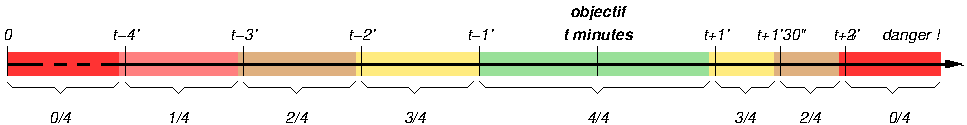
\includegraphics [width=\textwidth] {duree-prez.pdf}
    \end {center}
    \caption {Barème de la note (ici sur 4) en fonction de la durée
	de la présentation}
\end {figure}

%%%%%%%%%%%%%%%%%%%%%%%%%%%%%%%%%%%%%%%%%%%%%%%%%%%%%%%%%%%%%%%%%%%%%%%%%%%%%%
% Checklist mémoire
%%%%%%%%%%%%%%%%%%%%%%%%%%%%%%%%%%%%%%%%%%%%%%%%%%%%%%%%%%%%%%%%%%%%%%%%%%%%%%

\newenvironment{checklist}[1]{\vspace{-2.5ex}\section{#1}\vspace{-2ex}\begin{itemize}\vspace{-1ex}\small}{\end{itemize}}
\newcommand{\chkitem}[1]{\item [$\square$]#1}

\chapter {Checklist pour le mémoire}
    \label{checklist-mem}

Pour vous aider dans la rédaction du mémoire, voici une liste de
points à vérifier.  Une fois votre mémoire rédigé, vérifiez que
vous pouvez cocher \emph{toutes} les cases.

\begin{checklist}{Structuration du document}
\chkitem{Le titre du mémoire reflète ce que j'ai fait dans mon stage}
\chkitem{Le plan est clair et ne comporte pas d'allers-et-retours}
\chkitem{Les parties composant le mémoire sont de taille équilibrée}
\chkitem{Je respecte la limite de taille indiquée}
\chkitem{J'ai numéroté tous les chapitres, sections, sous-sections, etc. (1, 1.1, 1.1.1, etc.)}
\chkitem{J'ai numéroté toutes les pages (sauf la page de garde)}
\chkitem{Il y a une table des matières avec les numéros de page}
\chkitem{La lecture des annexes n'est pas nécessaire pour comprendre le travail que j'ai réalisé}
\chkitem{Tous les emprunts de texte/figure que j'ai faits sont dûment attribués à leurs auteurs respectifs}
\chkitem{Je mets l'accent sur la mise en œuvre des compétences attendues à mon niveau d'études, notamment l'esprit de synthèse, l'initiative et la maîtrise d'un problème complexe.}
\chkitem{Le maître de stage a validé mon mémoire}
\end{checklist}

\begin{checklist}{Présentation de l'entreprise}
\chkitem{J'ai présenté la structure d'accueil avec mes mots et j'ai évité de recopier un site web ou une plaquette commerciale}
\chkitem{La description de la structure d'accueil permet de comprendre son secteur d'activité, sa taille et son organisation}
\chkitem{Je donne des informations quantitatives lorsque cela permet de comprendre la dimension de la structure d'accueil et de son environnement}
\chkitem{Ma place dans la structure d'accueil est clairement explicitée et permet de comprendre les interactions avec mon environnement immédiat}
\end{checklist}

\begin{checklist}{Présentation des missions}
\chkitem{J'indique mes missions dès l'introduction, avant de les expliciter dans le reste du mémoire}
\chkitem{J'explicite la situation à mon arrivée, afin de bien faire comprendre la portée de ce que j'ai réalisé}
\chkitem{Je donne des informations quantitatives lorsque cela permet de comprendre la dimension du problème à résoudre}
\end{checklist}

\begin{checklist}{Présentation du travail effectué}
\chkitem{J'explicite les choix qui m'ont été imposés}
\chkitem{Je justifie tous les choix que j'ai effectués ou que j'ai contribué à effectuer}
\chkitem{En cas de travail partagé par plusieurs personnes, ma contribution personnelle est clairement explicitée}
\chkitem{Mon mémoire ne se limite pas à des descriptions techniques : je décris aussi les interactions avec les acteurs de mon stage : collègues, hiérarchie, clients, fournisseurs, prestataires...}
\chkitem{Plus que des étapes techniques, mon mémoire explicite la méthodologie que j'ai suivie}
\chkitem{Mes comparaisons sont plus claires avec un tableau de synthèse récapitulatif}
\chkitem{Je replace le travail effectué dans la stratégie de la structure d'accueil}
\end{checklist}

\begin{checklist}{Conclusions/réflexions}
\chkitem{Dans la conclusion, je donne des informations sur l'état du travail et son utilisation par la structure d'accueil}
\chkitem{Dans la conclusion, je donne des perspectives sur ce que pourrait être la suite du travail}
\chkitem{Je dresse le bilan des compétences acquises durant le stage, sans me limiter aux compétences techniques}
\end{checklist}

\begin{checklist}{Expression}
\chkitem{Je rédige le texte du mémoire et j'évite le style télégraphique ou les listes à puces sans phrases}
\chkitem{J'évite le style « parlé », chaque phrase comprend au moins un sujet, un verbe et un complément}
\chkitem{Je ne m'adresse pas directement au lecteur (« Je vais vous présenter mon travail »)}
\chkitem{Je ne passe pas à la ligne après chaque phrase et je respecte la règle « un paragraphe = une idée » }
\chkitem{Le texte de mon mémoire ne comprend aucun terme familier}
\chkitem{Je n'abuse pas des anglicismes : aucun des termes anglais restants n'a de traduction française bien acceptée}
\chkitem{J'utilise les verbes « permettre » et « pouvoir » à bon escient et avec parcimonie}
\chkitem{J'explicite les termes peu usuels}
\chkitem{J'emploie la première personne du singulier pour tout ce que j'ai fait moi-même}
\chkitem{J'emploie le présent ou le passé pour ce qui a été réalisé}
\chkitem{Je n'emploie le futur que pour ce qui n'est pas encore réalisé}
\chkitem{J'introduis les termes techniques ou les sigles peu courants en dehors de la structure d'accueil}
\chkitem{J'ajoute un lexique en fin de document pour récapituler les termes techniques ou les sigles lorsque j'en utilise beaucoup}
\end{checklist}

\begin{checklist}{Orthographe/grammaire}
\chkitem{J'ai passé le correcteur orthographique et grammatical... et j'ai corrigé les fautes}
\chkitem{J'ai fait relire le document par une personne maîtrisant l'orthographe et la grammaire}
\chkitem{Les URL figurant dans le mémoire (y compris dans la bibliographie) sont cliquables}
\end{checklist}

\begin{checklist}{Iconographie}
\chkitem{Chacune de mes figures est numérotée et légendée}
\chkitem{Les figures sont lisibles lorsqu'elles sont imprimées (sur papier) en noir et blanc}
\chkitem{Le texte dans les figures est de taille comparable au texte du mémoire}
\chkitem{Les copies d'écran ne comportant que du texte, les suites de commandes et les fichiers de configuration ne sont pas intégrés sous forme d'image, mais sous forme de texte}
\chkitem{Sauf cas particulier, toutes mes illustrations sont en format vectoriel}
\chkitem{Lorsque je ne peux pas faire autrement qu'intégrer une figure en « bitmap », je veille à ce qu'elle reste lisible}
\chkitem{Je ne place dans le mémoire que les figures indispensables à la compréhension}
\chkitem{J'indique les unités (appropriées) sur les graphiques}
\chkitem{J'ai cité chaque figure dans le corps du texte, avec une explication}
\chkitem{L'explication sur chaque figure indique bien ce que le lecteur est censé retenir de la figure}
\chkitem{Les concepts ardus ou les points spécifiques du stage sont illustrés avec des figures}
\end{checklist}

\begin{checklist}{Bibliographie}
\chkitem{J'ai ajouté une bibliographie pour que les personnes intéressées puissent approfondir certains sujets évoqués}
\chkitem{La bibliographie contient les références suffisantes pour accéder à tous les documents cités}
\chkitem{Tous les éléments référencés dans le texte sont indiqués dans la bibliographie}
\chkitem{Chaque élément de la bibliographie est cité au moins une fois dans le texte}
\end{checklist}

%%%%%%%%%%%%%%%%%%%%%%%%%%%%%%%%%%%%%%%%%%%%%%%%%%%%%%%%%%%%%%%%%%%%%%%%%%%%%%
% Checklist soutenance
%%%%%%%%%%%%%%%%%%%%%%%%%%%%%%%%%%%%%%%%%%%%%%%%%%%%%%%%%%%%%%%%%%%%%%%%%%%%%%

\chapter {Checklist pour la soutenance}
    \label{checklist-sout}

Comme pour le mémoire (voir annexe~\ref{checklist-mem},
page~\pageref{checklist-mem}), vous trouverez ci-après une liste de
points à vérifier pour réussir votre soutenance.

\begin{checklist}{Structuration}
\chkitem{Le titre de la présentation reflète ce que j'ai fait dans mon stage}
\chkitem{Le plan est clair et ne comporte pas d'allers-et-retours}
\chkitem{Les parties composant le diaporama sont de taille équilibrée}
\chkitem{La description de la structure d'accueil permet de comprendre le secteur d'activité, la taille, l'organisation, ainsi que l'environnement immédiat du stagiaire}
\chkitem{Ma place dans la structure d'accueil est clairement explicitée et permet de comprendre les interactions avec mon environnement immédiat}
\chkitem{Je donne des informations quantitatives lorsque cela permet de comprendre la dimension de la structure d'accueil et de son environnement}
\chkitem{Plus que des étapes techniques, j'explicite la méthodologie que j'ai suivie}
\chkitem{Le maître de stage a relu ma présentation}
\chkitem{J'ai répété ma présentation devant le maître de stage et j'ai intégré ses remarques}
\end{checklist}

\begin{checklist}{Présentation du contexte et des objectifs}
\chkitem{J'explicite la situation à mon arrivée, afin de bien faire comprendre la portée de ce que j'ai réalisé}
\chkitem{J'explicite les choix qui m'ont été imposés}
\chkitem{Je donne des informations quantitatives lorsque cela permet de comprendre la dimension du problème à résoudre}
\chkitem{J'introduis les termes techniques ou les sigles peu courants en dehors de la structure d'accueil}
\end{checklist}

\begin{checklist}{Présentation du travail réalisé}
\chkitem{Je justifie tous les choix que j'ai effectués ou que j'ai contribué à effectuer}
\chkitem{En cas de travail partagé par plusieurs personnes, ma contribution personnelle est clairement explicitée}
\chkitem{Je replace le travail effectué dans la stratégie de la structure d'accueil}
\end{checklist}

\begin{checklist}{Bilan, conclusion, réflexions}
\chkitem{Dans la conclusion, je donne des informations sur l'état du travail et son utilisation par la structure d'accueil}
\chkitem{Dans la conclusion, je donne des perspectives sur ce que pourrait être la suite du travail}
\chkitem{Je dresse le bilan des compétences acquises durant le stage, sans me limiter aux compétences techniques}
\end{checklist}

\begin{checklist}{Qualité des diapos}
\chkitem{Les diapos ne sont ni trop remplies, ni trop vides}
\chkitem{Le diaporama comporte du texte et des illustrations de manière équilibrée}
\chkitem{Le texte des diapos correspond à des points clefs, et non à des phrases complètes}
\chkitem{Tous les messages à destination de l'assistance sont explicités}
\chkitem{Tous les emprunts de texte/figure que j'ai faits sont dûment attribués à leurs auteurs respectifs}
\chkitem{J'ai passé le correcteur orthographique et grammatical... et j'ai corrigé les fautes}
\chkitem{J'ai fait relire le document par une personne maîtrisant l'orthographe et la grammaire}
\chkitem{Les diapos sont numérotées}
\chkitem{Les diapos sont sur un fond clair (ou mieux : blanc)}
\chkitem{Le diaporama comporte de nombreuses illustrations pour mieux faire comprendre les points délicats}
\chkitem{Mes illustrations véhiculent une idée ou un message à faire passer à l'auditoire, que j'explicite au moins oralement}
\chkitem{J'illustre avec des schémas les concepts ardus ou les points spécifiques de mon stage}
\chkitem{Dans les figures, les couleurs doivent être contrastées car la projection aplatit les couleurs}
\chkitem{Lors de la projection, le texte et les figures doivent pouvoir être lus au 5e rang de la salle}
\chkitem{Le texte dans les figures est de taille comparable au texte des diapos, et il reste lisible au 5e rang}
\chkitem{Les copies d'écran ne comportant que du texte, les suites de commandes et les fichiers de configuration ne sont pas intégrés sous forme d'image, mais sous forme de texte}
\chkitem{Lorsque je ne peux pas faire autrement qu'intégrer une figure en «~bitmap~», je veille à ce qu'elle reste lisible}
\chkitem{Sauf cas particulier, toutes mes illustrations sont en format vectoriel}
\chkitem{J'explicite les termes peu usuels}
\chkitem{Mes comparaisons sont plus claires avec un tableau de synthèse récapitulatif}
\end{checklist}

\begin{checklist}{Gestion du temps}
\chkitem{Je présente le plan}
\chkitem{Le temps est compté : plus long, c'est une pénalité}
\chkitem{Le temps est compté : plus court, c'est courir le risque de manquer de matière}
\chkitem{Je ne passe pas plus d'une minute ou deux par diapo}
\end{checklist}

\begin{checklist}{Élocution, discours, posture}
\chkitem{Ma tenue vestimentaire est adaptée au moment solennel que constitue la soutenance}
\chkitem{Je ne prends pas mes notes avec moi}
\chkitem{Je regarde l'assistance, et non mes notes ou mes diapos (sauf pour pointer un élément important)}
\chkitem{Je suis enthousiaste, je souris}
\chkitem{Je parle assez fort et distinctement}
\chkitem{J'impulse un rythme dynamique à mon discours}
\chkitem{Je fais attention à ne pas utiliser un langage familier}
\chkitem{Je fais attention à mes tics verbaux («~du coup~», «~en fait~»...)}
\chkitem{Je fais attention à ma posture : je ne me fige pas, mais je ne gigote pas}
\chkitem{J'emploie la première personne du singulier pour tout ce que j'ai fait moi-même}
\chkitem{J'emploie le présent ou le passé pour ce qui a été réalisé}
\chkitem{Je n'emploie le futur que pour ce qui n'est pas encore réalisé}
\chkitem{Je n'abuse pas des anglicismes : aucun des termes anglais que j'utilise n'a de traduction française bien acceptée}
\end{checklist}

\begin{checklist}{Réponses aux questions}
\chkitem{Une fois la présentation terminée, je laisse la projection active au cas où une question ferait référence à une diapo}
\chkitem{Je laisse les membres du jury terminer de poser leur question avant de commencer à répondre}
\chkitem{En cas de doute, je reformule la question pour être sûr de l'avoir bien comprise et ne pas risquer de répondre à côté}
\chkitem{Si je ne sais pas répondre à une question, je préfère dire que je ne sais pas plutôt que de répondre n'importe quoi}
\end{checklist}

%%%%%%%%%%%%%%%%%%%%%%%%%%%%%%%%%%%%%%%%%%%%%%%%%%%%%%%%%%%%%%%%%%%%%%%%%%%%%%
% Bibliographie
%%%%%%%%%%%%%%%%%%%%%%%%%%%%%%%%%%%%%%%%%%%%%%%%%%%%%%%%%%%%%%%%%%%%%%%%%%%%%%

\cleardoublepage
\bibliographystyle{plain}
\bibliography{memoire}

\end{document}
